% Oppsett, ikke noe å bry seg om.
\documentclass[12pt,norsk,a4paper]{article}
\usepackage{graphicx}
\usepackage{hyperref}
\usepackage{float}
\usepackage{pdfpages}
\usepackage{ulem}
\usepackage[utf8]{inputenc}
\usepackage[norsk]{babel}
\usepackage{multirow}
\usepackage{colortbl}
\usepackage{array}

\begin {document}
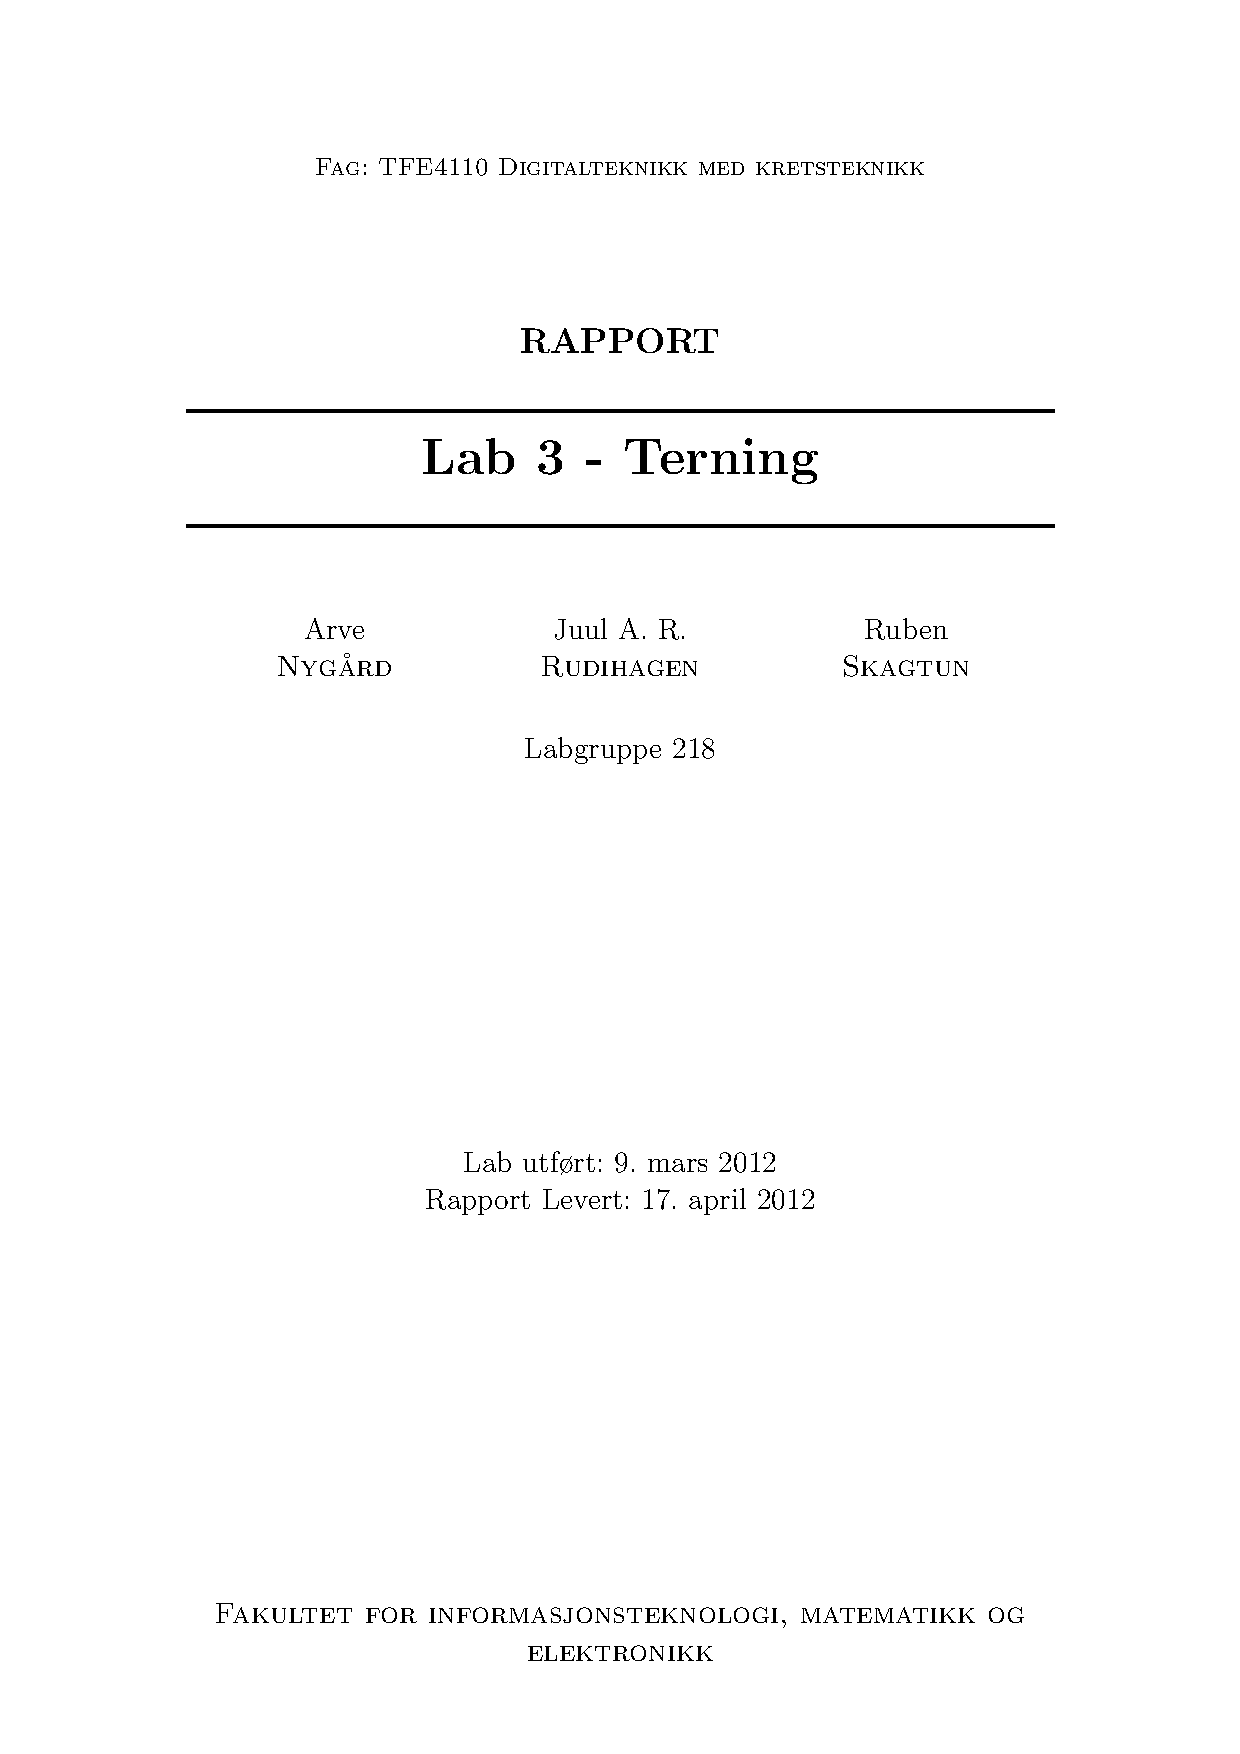
\includepdf{titlepage}
\clearpage



\section*{} % Stjerne etter section -> Siden tas ikke med når latex teller sidetall
\thispagestyle{empty}   
\begin{center}
\Large \textsc{Labrapport: Lab 3 - Terning}
\end{center}
\clearpage

\section*{Sammendrag}
\thispagestyle{empty}  

I denne rapporten blir det beskrevet hvordan gruppen utførte en laboppgave hvor målet var å lage en digital krets, ved hjelp av diskrete portkretser, som styrer lysdioder slik at de danner mønstrene til en vanlig sekssidet terning. Et viktig poeng er at terningen skal ha en uniform verdidistribusjon, slik at den oppfører seg som en virkelig terning.\\
\\
Etter å ha kommet frem til et design på papiret, ble kretsene loddet opp og testet. Gruppen fikk produsert to kretser som viste tilfeldige terningmønstre, som etter 60 testkjøringer viste seg å ha en uniform distribusjon av verdier. Et tredje kretskort ble startet på, men ikke fullført i tide.
\clearpage

\tableofcontents %Innholdsfortegnelse. Genereres automatisk. :)
\thispagestyle{empty}   
\clearpage

\section{Innledning} 
\setcounter{page}{1}
I dette eksperimentet skal gruppen designe, koble opp, og teste en digital krets som representerer en terning. Det skal først lages en skjematisk fremstilling av kretsen [fig. \ref{fig:kretskortet}], før denne loddes opp med fysiske komponenter. \\
\\
Terningen skal fungere på følgende måte: Du trykker ned en knapp for å rulle terningen. Når knappen er presset inn, vil tallgeneratoren rullere mellom verdiene 1-6, med svært høy hastighet. Når knappen slippes, stopper generatoren opp på nåværende tall, og vises ved hjelp av lysidodene. Det er kritisk at tallgeneratoren rullerer mellom verdier raskt nok til at det blir umulig for et menneske å forutsi hvilken verdi vil få.\\
\\
Terningen består av tre hoveddeler [fig. \ref{fig:blokkskjema}]: En tilfeldig tallgenerator, logikk som konverterer tallet til et mønster, og lysdioder som viser dette mønsteret. Virkemåten til disse delene er forklart under teoridelen av rapporten.


\clearpage

\section{Teoretisk grunnlag}
Terningen består av tre hoveddeler som vi skal forklare hvordan fungerer. Det er en tilfeldig tallgenerator som til enhver tid
gir ut et trebits binærtall mellom 001 og 110, som er henholdsvis 1 og 6. Logikken skal så oversette denne tallrekken til et nytt firebits binærmønster som styrer lysdiodene. Til slutt er lysdiodene som lyser et tall mellom en og seks som vist på en terning. Se figur under:
\begin{figure}[H]
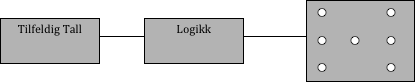
\includegraphics{Blokkskjema.png}
\caption{Hoveddelene til terningen}
\label{fig:blokkskjema}
\end{figure}

    \subsection{Tilfeldig tallgenerator}
    Den tilfeldige tallgeneratoren baser en teller som teller fra 1 til 6 i en evig loop. Dette skjer vet at når telleren overstiger verdien seks begynner den å telle på en igjen. Telleren blir klokket av en oscillator som svinger
    veldig raskt, dette gjør at verdien til telleren skifter så fort at vi kan si det er tilfeldig hvilket tall som kommer ut når man slipper bryteren. Denne oscillatoren består av en NAND- og en NOR-port, i tillegg til noen motstander og kondensatorer. Se figur under:
    \\
    \\
    \textbf{Her burde vi kanskje ha et bilde?} 

    
    \subsection{Lysdioder}
    Lysdiodene på kretskortet som vi bruker til å vise hvilket tall terningen får er aktiv lave. Det vil si at dersom de får inn '0'
    så vil de lyse. Selv om dette kan virke forvirrende er det hensiktsmessig fordi det fører til at vi får mindre indre motstand. Dette fører igjen til at vi får mer strøm som gir sterkere lys. For å gi ut alle tallene en terning kan gi, ved en mest mulig lik tilnærming trenger vi 7 lysdioder og 4 styresignal. Grunnen til at vi bare trenger 4 styresignal til 7 lysdioder er fordi noen av dem kan kontroleres med samme styresignal. Hvilket dioder som lyser samtidig er markert på figuren under:

    \begin{figure}[H]
    \begin{center}
    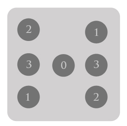
\includegraphics[scale=1]{Terning.png}
    \caption{Figur av terninen. Diodene med samme nummer lyser alltid samtidig}
    \label{fig:terning}
    \end{center}
    \end{figure}

    \subsection{Logikken}
    Logikken sin oppgave er å oversette signalene Q2-Q0 som representerer den binære verdien til hvilket tall terningen skal gi, til styresignalene S3-S0 som styrer lysene på terningen. Et poeng er å gjøre kretsen så effektiv som mulig, for å oppnå dette brukte vi Karnaugh-Diagram. Utledningen som ble gjørt er lagt ved som Vedlegg 1 og Vedlegg 2. En kort oppsumering av resultatet vises i tabellen under.

    \begin{table}[H] 
    \begin{center}
        \begin{tabular}{ | c | l |} 
        \hline
        $Styresignal$  & $Logisk uttrykk$ \\ \hline 
        S0 & $\neg Q_0$\\ \hline
        S1 & $\neg Q_2 \wedge \neg Q_1$\\ \hline
        S2 & $\neg Q_2$\\ \hline
        S3 & $\neg Q_2 + \neg Q_1$\\ \hline
        \hline
        \end{tabular}
        \end{center}
        \caption{Tabell på hvordan logikken konverterer ingangsbittene til styresignalene}

\end{table}

    Ut fra denne tabellen kan vi sette opp hvordan den totale kretsen skal bli når vi kobler den sammen. Resultatet er fremstil på bilde under: 

    \begin{figure}[H]
    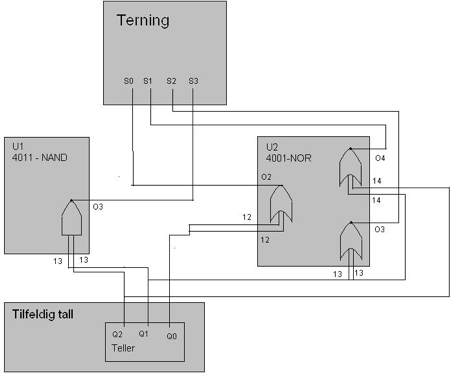
\includegraphics[scale=0.75]{Krestkortet.png}
    \caption{Sammenhengen mellom bitverdiene og styresignalende}
    \label{fig:kretskortet}
    \end{figure}

    Som en ser på bilde har vi lagd inverterere ved å koble samme inngangsignal i begge inngangene på en NAND- eller NOR-port. Vi kunne oppnådd samme effekt dersom vi koblet en av inngangene til jord.    

\clearpage

\section{Målemetode og arbeidsbeskrivelse}
Forarbeidet til denne laboratorieøvelsen leder en frem til et ferdigstilt og fungerende kretskort som genererer tallene til en terning, med andre ord, tall mellom en og seks. Selve laboratoriedelen består av lodding og sammenkobling av tallgeneratoren og diodene.
\\
\\
Det aller første som må gjøres i denne laben er å lodde på alle komponentene til et av krestkortene. En må lodde opp diodene, IC-soklene, motstander osv. Når dette er gjort er en nødt til å bruke oscilloskopet til å kontrollere at tallgeneratoren fungerer (Se vedlegg 3). Bruk probe 'auto-check' på alle utgitte prober og se til at de alle får en melding om 'passed'. For å kontrollere at tallgeneratoren fungerer bruker en proben som er utgitt på labplassen. Koble proben opp mot oscilloskopet og gjennomfør målingene ved å holde proben inntil pinne 3 på U2. Hold deretter proben inntil 
\clearpage


\section{Utstyrsliste} 
    \begin{itemize} 
    \item Kretskort

Serienumber: ZBX0512.169630-423
    \item Spenningskilde

Enhetsnummer: 74
    \item Plassnummer 47
    \item Multimeter

Enhetsnummer: 37
    \item Loddebolt

Enhetsnummer: 59
    \item Oscilloskop

Serienumber: G04-0281

    \end{itemize}
\clearpage


\section{Resultater}
Gruppen fikk ferdigstilt og testet to terningkretser. Terningene er konstruert for å drives av en 5V spenningskilde, men gruppen rakk ikke å lage en batteriadapter. 



Tabell [\ref{tbl:probabilitetsdistribusjon}] viser resultatet av 60 kast.
\begin{table}[H]
    \begin{center}
    \begin{tabular}{|c|c|}
    \hline
    Verdi & Antall ganger\\ \hline
    1 & 13 \\ \hline
    2 & 8  \\ \hline
    3 & 10 \\ \hline
    4 & 8  \\ \hline
    5 & 10 \\ \hline
    6 & 11 \\ \hline
    \end{tabular}
    \caption{Probabilitetsdistribusjon etter 60 'kast' på den første terningen.}
    \label{tbl:probabilitetsdistribusjon}
    \end{center}
    \end{table}


\begin{table}[H]
    \begin{center}
    \begin{tabular}{|c|c|c|}
    \hline
    Pinne & $\frac{T_H}{T_D}$ (ms) & Probabilitet   \\[1mm] \hline
    $S_0$ & $\frac{1.13}{2.26}$  & $\frac{1}{2}$    \\[1mm] \hline
    $S_1$ & $\frac{1.13}{6.78}$  & $\frac{1}{6}$    \\[1mm] \hline
    $S_2$ & $\frac{3.39}{6.78}$  & $\frac{1}{2}$    \\[1mm]\hline
    $S_3$ & $\frac{5.65}{6.78}$  & $\frac{5}{6}$    \\[1mm] \hline
    \end{tabular}
    \caption{Probabilitetsdistribusjon for pinnene $S_0 - S_3$  på kretsen som styrer lysdiodene}
    \label{tbl:probe}
    \end{center}
    \end{table}

\clearpage

\section{Diskusjon}
Resultatet bekrefter at implementeringen er rett, de 60 kastene ble så jevnt fordelt som vi kunne for vente med så få kast. Vår analyse av utgangssignalene $S_0 - S_3$ (tabell \ref{tbl:probe})ble akkurat som forventet ut ifra forarbeidet. Som en kan se i tabell [\ref{tbl:probabilitetsdistribusjon}], fikk vi alle kombinasjoner av øyne som en terning kan gi, og ingen ulovlige verdier. Vi anser det som at implementeringen av terningen var vellykket, og at det ikke er noen defekte deler eller feil i logikken. 


\clearpage

\section{Konklusjon}


\clearpage

\section{Vedlegg}
    \subsection{Vedlegg 1: sammenheng mellom binærverdi og styresignal.}
    \begin{table}[H]
    \begin{center}
    \begin{tabular}{|c|c|c|c|c|c|c|c|c|}
    \hline
    Hex & \multicolumn{3}{c}{Binærverdi} & \multicolumn{4}{|c|}{Styresignal}&hex \\ \hline
    $Q$ & $Q_2$ & $Q_1$ & $Q_0$ & $S_3$ & $S_2$ & $S_1$ & $S_0$ & $S$ \\ \hline
    0 & 0 & 0 & 0 & X & X & X & X & - \\ \hline 
    1 & 0 & 0 & 1 & 1 & 1 & 1 & 0 & E \\ \hline
    2 & 0 & 1 & 0 & 1 & 1 & 0 & 1 & D \\ \hline
    3 & 0 & 1 & 1 & 1 & 1 & 0 & 0 & C \\ \hline
    4 & 1 & 0 & 0 & 1 & 0 & 0 & 1 & 9 \\ \hline
    5 & 1 & 0 & 1 & 1 & 0 & 0 & 0 & 8 \\ \hline
    6 & 1 & 1 & 0 & 0 & 0 & 0 & 1 & 1 \\ \hline
    7 & 1 & 1 & 1 & X & X & X & X & - \\ \hline
    \end{tabular}
    \end{center}
    \caption{Resultat $S_0=\neg Q_0$}
    \end{table}
    \clearpage

    \subsection{Vedlegg 2: Karnaugh-Diagram}
    \begin{table}[H]
    \begin{center}
    \begin{tabular}{|l|l|r|r|} \hline
    \multicolumn{4}{|c|}{Tabell for $S_0$} \\ \hline
    $Q_2$ & $Q_1$ & \multicolumn{2}{|r|}{$Q_0$ \hspace{20 mm} 0 \hspace{2 mm} 1} \\ \hline
    0 & 0 & \hspace{27 mm} X \cellcolor[gray]{0.8} & 0 \\ \hline 
    0 & 1 & 1 \cellcolor[gray]{0.8} & 0 \\ \hline
    1 & 1 & 1 \cellcolor[gray]{0.8} & X \\ \hline
    1 & 0 & 1 \cellcolor[gray]{0.8} & 0 \\ \hline
    \end{tabular}
    \end{center}
    \label{juul}
    \caption{Resultat $S_0=\neg Q_0$}
    \end{table}

    \begin{table}[H]
    \begin{center}
    \begin{tabular}{|l|l|r|r|} \hline
    \multicolumn{4}{|c|}{Tabell for $S_1$} \\ \hline
    $Q_2$ & $Q_1$ & \multicolumn{2}{|r|}{$Q_0$ \hspace{20 mm} 0 \hspace{2 mm} 1} \\ \hline
    0 & 0 & \hspace{27 mm} X \cellcolor[gray]{0.8} & \cellcolor[gray]{0.8} 1 \\ \hline 
    0 & 1 & 0 & 0 \\ \hline
    1 & 1 & 0 & X \\ \hline
    1 & 0 & 0 & 0 \\ \hline
    \end{tabular}
    \end{center}
    \caption{Resultat $S_1=\neg Q_2 \wedge \neg Q_1$}
    \end{table}


    \begin{table}[H]
    \begin{center}
    \begin{tabular}{|l|l|r|r|} \hline
    \multicolumn{4}{|c|}{Tabell for $S_2$} \\ \hline
    $Q_2$ & $Q_1$ & \multicolumn{2}{|r|}{$Q_0$ \hspace{20 mm} 0 \hspace{2 mm} 1} \\ \hline
    0 & 0 & \hspace{27 mm} X \cellcolor[gray]{0.8} & \cellcolor[gray]{0.8} 1 \\ \hline 
    0 & 1 & 1 \cellcolor[gray]{0.8} & 1 \cellcolor[gray]{0.8} \\ \hline
    1 & 1 & 0 & X \\ \hline
    1 & 0 & 0 & 0 \\ \hline
    \end{tabular}
    \end{center}
    \caption{Resultat $S_2=\neg Q_2$}
    \end{table}

    \begin{table}[H]
    \begin{center}
    \begin{tabular}{|l|l|r|r|} \hline
    \multicolumn{4}{|c|}{Tabell for $S_0$} \\ \hline
    $Q_2$ & $Q_1$ & \multicolumn{2}{|r|}{$Q_0$ \hspace{20 mm} 0 \hspace{2 mm} 1} \\ \hline
    0 & 0 & \hspace{27 mm} X \cellcolor[gray]{0.8} & \cellcolor[gray]{0.8} 1 \\ \hline 
    0 & 1 & 1 \cellcolor[gray]{0.8} & 1 \cellcolor[gray]{0.8} \\ \hline
    1 & 1 & 0 & X \\ \hline
    1 & 0 & 1 \cellcolor[gray]{0.8} & 1 \cellcolor[gray]{0.8} \\ \hline
    \end{tabular}
    \end{center}
    \caption{Resultat $S_3=\neg Q_2 + \neg Q_1$}
    \end{table}
\clearpage

    \subsection{Vedlegg 3: Oscillatorbilder}
    \begin{figure}[H]
    \begin{center}
    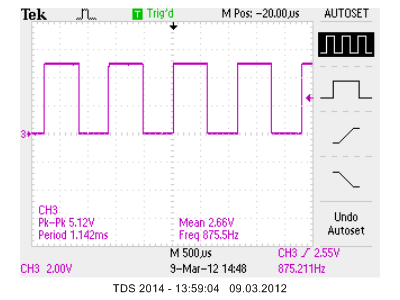
\includegraphics[scale=1.0]{Fig1.png}
    \caption{Oscillatorfrekvens målt på pinne 3 på U2.}
    \end{center}
    \label{fig:Oscillatorbilde1}
    \end{figure}

    \begin{figure}[H]
    \begin{center}
    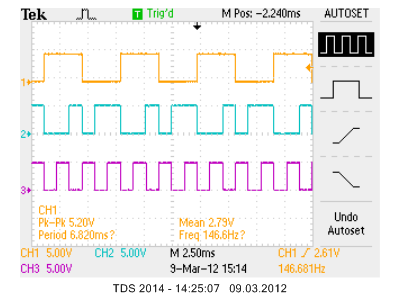
\includegraphics[scale=1.0]{Fig2.png}
    \caption{Måling med probene Q2, Q1 og Q0.}
    \end{center}
    \label{fig:Oscillatorbilde2}
    \end{figure}


\clearpage

\section{Litteraturhenvisninger}
\clearpage

\section{Tilbakemeldinger}
Det hadde vært kjekt om det var klargjort batteriadapter til denne oppgaven. Enten bare en ferdiglaget adapter, eller at dette ble tatt med som en del av oppgaven. Kanskje designet av en kunne vært med som forhåndsoppgave.\\
\\
Ellers synes alle på gruppen at dette var en morsom lab! Kjekt å få med seg en selvprodusert digital terning hjem!
\clearpage
\end{document}